In the Chapter \ref{ch:usbe_lung} we introduced the problem of
\ac{DUS}-induced lung hemorrhage, however the focus was on the
fundamental physical problem of an acoustically driven gas-liquid
interface, such as those of the alveoli. In this chapter we aim to
extend that work to increase its relevance to \ac{DUS} of the
lung. Here, I hypothesize that \ac{DUS} may be capable of generating
sufficient baroclinic vorticity at alveolar interfaces in the lung to
drive deformation and hemorrhage. To investigate this hypothesis I
examine the dynamics of water-air interfaces driven by ultrasound
pulses and compute relevant stresses and strains at the interface for
comparison to expected damage thresholds based on previous research.

\section{Introduction}
Lung \ac{US} has become a common tool for imaging and diagnostics in
critical and point-of-care situations and its use is growing
\citep{Lichtenstein2009}. Currently, \ac{PH} is the only biological
effect known to occur in mammals as a result of non-contrast
diagnostic ultrasound and it has been shown to occur under clinically
acceptable parameters with \ac{MI}$\leq1.9$ \citep{FDA1997} and peak
pressures as low as $1$ MPa \citep{Dalecki1997}. The physical
mechanism underlying this damage is still not well understood. And
while the occurrence of hemorrhage as a result of diagnostic lung
\ac{US} has not been directly studied in human lungs for obvious
ethical reasons, an understanding of the underlying cause is important
for the development of safe guidelines and procedures.

In Chapter \ref{ch:usbe_lung}, the body of literature covering
research into the physical mechanisms of \ac{DUS} was reviewed, so
only a brief summary will be provided here. Pulmonary damage induced
by pulsed ultrasound is characterized by hemorrhage of plasma proteins
and erythrocytes into the alveoli \cite{Penney1993a}. Alveolar edema
or frank hemorrhage has also been shown to occur as a result of
mechanical stress failure of the alveolar membrane induced by over
pressure \citep{West1991}. \ac{DUS}-induced hemorrhage in the lungs
appears mechanical in nature and thermal mechanisms appear unlikely
\citep{Zachary2006, Dalecki2004}. Among possible mechanical damage
mechanisms cavitation, acoustic radiation force, acoustic fountaining
or atomization have all been considered. Experimental results suggest
that neither inertial cavitation nor radiation force can completely
explain the damage \citep{OBrien2000, Raeman1996, Miller2016}. This
work aims to use numerical experiments to investigate the stresses and
strains imparted by an ultrasound pulse on a perturbed liquid-gas
interface, such similar to those of the alveoli.

The anatomical structure of the lungs has been studied extensively and
is of particular interest to the present work. The alveoli can be
thought of as a network of openly connected, air-filled saccules with
distinctly irregular surfaces. And while alveoli are irregularly
shaped and do not have a true diameter, past research suggests that
their size appears to be species dependent \citep{Faffe2002}. Mean
alveolar diameters range from tens to hundreds of microns with
reported values of 45 $\mu$m in mice \cite{Knust2008} and 200 $\mu$m
in adult humans \cite{Ochs2004} for examples. The septa that separate
adjacent alveoli are nearly planar structures that contain several
tissue layers and are coated with a thin layer of liquid surfactant
\citep{Gil1979,Reifenrath1975,Perlman2014}. Among the tissue layers
surrounding the alveoli is a sheet-like web of blood-filled
capillaries. These pulmonary capillaries are almost completely
unsupported by surrounding tissue \cite{West1991}. Separating the
blood from the air is a multi-layer wall of tissues, $0.2$ - $0.3\mu$m
thick, referred to as the blood-gas or \ac{BAB} \citep{West2000}. The
extreme thinness of this barrier is necessary for efficient gas
exchange. The physical dimensions of the alveolus and thinness of this
barrier relative to typical \ac{US} wavelengths are of importance to
the model used in this study.

In addition to anatomical structure, the mechanical properties and
failure behavior of alveoli and other relevant pulmonary tissues have
been studied extensively in computational and animal
models. \cite{Perlman2014} combined experimentally measured strains
with computationally modeled lung stresses to demonstrate that the
effective Young's moduli of aveolar septa depend on transpulmonary
pressure. Values range from $E_a=12$ kPa at a low transpulmonary
pressure around $0.4$ kPa to $E_a=140$ kPa at a high transpulmonary
pressure of approximately $2$ kPa. \cite{West1991} raised the
pulmonary capillary pressure of anesthetized rabbits and observed
consistent stress failure of the capillary and alveolar epithelium for
transmural at or above $40$ mmHg ($5.3$ kPa). This failure
corresponded to a $\sim25$ mN/m wall tension in the capillaries, which
is ``comparable with the tension in the alveolar wall''. The capillary
wall stress at failure was calculated to be approximately $8$
kPa. \begin{comment}
  This is roughly consistent with \cite{Welling1972} which measured
  properties of basement membranes from rabbit renal tubules and
  showed that a $57 \mu$m tubule could withstand $4.1$ kPa transmural
  pressure, which, based on a Laplace relationship, equates to an
  ultimate tensile strength of 500 kPa \citep{West1999}. Furthermore,
  \cite{Welling1972} also showed that properties of these tubules
  depended only on the strength of their basement membrane.
\end{comment}

Alveolar strain response has also been previously studied. Linear,
alveolar strain due to normal tidal breathing is in the range of
$0$-$5$\% \citep{Roan2011}. And \cite{Vlahakis2000} reports that
alveolar plasma membranes resist lateral tension and fail under
stresses greater than $0.4-0.6$ Pa, which corresponds to strains of
$2-3\%$. However, this work also acknowledges that typical changes in
cellular surface area are primarily a result of plasma membrane
unfolding and not actual wall strain. \citep{Belete2010} found that
when subjected to cyclical linear stretch at 0.5 Hz for 30 minutes,
rat alveolar epithelial cells experiencing Linear strains of $8\%$ or
greater were frequently damaged, whereas those experiencing strains
of $3 - 6\%$ often undamaged. 

Based on the work the previous chapter and the past research of
alveolar stress and strain failure we investigate the role of pulsed
ultrasound in possible stress and strain failure of alveoli. In this
chapter numerical experiments to simulate the dynamics of gas-liquid
interfaces driven by ultrasound pulse waveforms within the clinically
relevant range. Specifically, based on the work of Chapter
\ref{ch:usbe_lung}, I look for vorticity driven strains of the
interface, and establish simple models for computing the associated
passive viscous and elastic stresses. The computed stresses and
strains are compared to established failure criteria for alveoli to
access the relevance of this work to \ac{DUS} induced lung hemorrhage.


%%%%%%%%%%%%%%%%%%%%%%%%%%%%%%% 
\section{Methods}
Much of the basic problem setup, computational framework, and solution
setup laid out in Chapter \ref{ch:usbe_lung} are used here. In this
section I will focus specifically on three specific areas where
changes have been made to increase the relevance of the problem to
diagnostic ultrasound: (1) Problem geometry, (2) The acoustic wave,
(3) The calculation of stress and strain.

\subsection{Problem geometry}
In the previous section, we simulated trapezoidal acoustic waves
impinging upon a nearly planar interface with a sinusoidal
perturbation. The width of the domain represents a signle alveolar
diameter, $\ell$. The amplitude $a_0$ of this pertubation was $0.03\%$
its wavelength, again $\ell$, and for the sake of our simulation
corresponds $3\%$ the diameter of an alveolus. This implies a nearly
flat alveolar surface, which as we can see is not always the case,
based on the histological cross section of alveoli shown in Figure
\ref{fig:alveolar_histology}. To account for the variety of geometries
in alveolar tissue, many of which are not particularly flat, I will
now also consider perturbation amplitudes of $a_0=0.1\ell$ and
$a_0=0.3\ell$. I note that this in no way accounts for the range of
cross-sectional alveolar geometries that can exist, but we are limited
by computational constraints and our ability to resolve small scale
features that appear for larger perturbations and sharper geometries.
\begin{figure}
  \centering
  \begin{subfigure}[b]{0.45\textwidth}
    \includegraphics[width=\textwidth]{./figs/lung_figs/alveolar_sac}
    \caption{\label{fig:alveolar_histology}A histological cross section of alveoli. [By Jpogi (Own work) [CC BY-SA 4.0
      (http://creativecommons.org/licenses/by-sa/4.0)], via Wikimedia
      Commons]}
  \end{subfigure}
  % ~
  % \begin{subfigure}[b]{0.45\textwidth}
  %   \centering
  %   \includegraphics[width=\textwidth]{./figs/lung_figs/problem_schematic}
  %   \caption{\label{fig:ic_schematic}\hl{(STILL TO BE MODIFIED)}A
  %   schematic view of the model problem.}
  % \end{subfigure}
  \caption{A cross sectional view of alveolar tissue \protect\subref{fig:alveolar_histology}}
\end{figure}
% 
\subsection{Modeling the diagnostic ultrasound pulse}
The diagnostic ultrasound pulse is modeled as a sinusoidal carrier
wave of amplitude $p_a$ and frequency $f$ modulated by a Gaussian
Envelope such that,
\begin{align}
  p(x,t_0) = p_a\sin{\left(2\pi f\frac{\left[y-\left(Y_{wave}+L_{wave}\right)\right]}{c}\right)}\exp{\left(-\frac{\left(\left[y-\left(Y_{wave}+L_{wave}/2\right)\right]c\right)^2}{FWHM/\left(2\sqrt{2\ln{\left(2\right)}} \right)}\right)}.%
\end{align}
\begin{figure}
  \centering
%  \begin{subfigure}[b]{0.45\textwidth}
    \def\svgwidth{0.5\textwidth}
    \import{./figs/lung_figs/}{p0_vs_t_us_general.pdf_tex}%
%    \includegraphics[width=\textwidth]{./figs/lung_figs/}
    \caption{\label{fig:alveolar_histology} Sample ultrasound pulse waveform}
%  \end{subfigure}
\end{figure}

The carrier wavelength $\lambda=c_{water}/f$ and the full width of the
Gaussian envelope at half of the maximum amplitude ($FWHM$) are
designed to scale appropriately with respect to $\ell$. Here, we
choose design parameters of $f\approx 1.25 c_{water} / 2\pi \ell$ and
$FWHM=15\ell$ such that for an alveolar length scale of
$\ell=200 \mu$m, the corresponding center frequency is $f=1.65$ MHz
and $FWHM=3$ mm. $L_{wave}=45\ell$ is the length of the portion of the
computational domain, over which the wave is defined to exist, such
that the approximate duration of the wave-interface interaction is
just under $6 \mu$s. $Y_{wave}$ is $y$-location of the bottom of the
wave at $t=0$, which is set to $10a_0$ above the peak of the
interface. To consider the dependence of the interface dynamics on
pulse amplitude within the relevant range we vary $p_a = 1, 2.5,$ and
$5$ MPa.

\subsection{Stress and strain at the alveolar interface}%
\label{subsec:usbe_lung_bio_stress_strain}
To interpret the results of the numerical experiments to be performed
in the context of \ac{DUS}-induced lung injury, we aim to compare to
accepted stress and strain injury criteria for lung tissue. To do this
we calculate the strain of the air-water interface and the passive
viscous stress in the field. We note that from the available strain
and strain rate data, it would be possible to compute a passive total
viscoelastic stress at the interface if an acceptable constitutive
model were available. However, constitutive models appropriate to this
work do not appear available at this time and the development of such is beyond the scope of
this dissertation. For sake of justification of the model, a simple
model for estimating the order of magnitude of the involved elastic
forces can be found in \ref{app:lung_elastic}

\paragraph*{Calculation of the viscous stress}
We aim to calculate an approximate viscous stress, however because we
solve the Euler equations our simulations are inherently of an
inviscid flow. We do this because, while the justifications in Chapter
\ref{ch:usbe_lung} suggest that flow dynamics can be reasonably
approximated by neglecting viscosity, to understand the results in the
context of alveolar injury, an understanding of the approximate
viscous stress associated with \ac{DUS} is essential. To do this, we
calculate a passive viscosity at each point in space and time as
$\mu(x,y,t)$ based on the physical properties of air and water, and
the volume fraction of water $\alpha(x,y,t)$ such that
$\mu = \alpha\mu_{water} + (1-\alpha)\mu_{air}$. The shear stress for
a two-dimensional, Newtonian flow is calculated using the computed
viscosity field and the velocity gradients as
\begin{align}
  \tau_{xy}(x,y,t) = \mu\left(\frac{du}{dy}+ \frac{dv}{dx}\right).
\end{align}
The maximum viscous stress is extracted from the field. As will be
shown, this maximum occurs as the interface and as such, it will be
compared to relevant stress failure criteria.
%
\begin{comment}
  \begin{align}%
    \tau_{ij}=\mu%
    \begin{bmatrix}%
      0 & \frac{du}{dy}+\frac{dv}{dx}\\%
      \frac{dv}{dx}+\frac{du}{dy} & 0%
    \end{bmatrix}%
  \end{align},
\end{comment}
%
\paragraph*{Calculation of the interface strain}
The interface strain is calculated as 
\begin{align}%
  \label{eq:linear_strain}%
  \varepsilon = \frac{s(t) - s_0}{s_0}
\end{align}
where $s$ is the arc length of the interface.  This is consistent with
previous alveolar strain calculations by \cite{Roan2011}, which used
the relative change in alveolar diameters, which is analagous to the
interface arc length here.

%%%%%%%%%%%%%%%%%%%%%%%%%%%%%%% 
\section{Results and Discussion}
Simulations of interactions between sinusoidally perturbed water-air
interfaces and diagnostic ultrasound pulses were performed for wave
amplitudes of $p_a=1$, $2.5$, and $5$ MPa and initial perturbation
amplitudes of $a_0=0.03\ell$, $0.1\ell$ and $0.3\ell$.

\subsection{Qualitative observations of the interface}
Figures \ref{fig:rho_snapshots_A10}, \ref{fig:rho_snapshots_A25}, and
\ref{fig:rho_snapshots_A50} show density contour snapshots of the
interface for pulse amplitudes of $1, 2.5,$ and $5$ MPa respectively
at dimensionless times $t=1, 10, 100,$ and $500$. In each case,
subfigures \subref{fig:rho_snapshot_03}, \subref{fig:rho_snapshot_10},
and \subref{fig:rho_snapshot_30} correspond to initial perturbation
amplitudes of $a_0=0.03\ell, 0.1\ell,$ and $0.3\ell$ respectively. For
a $200 \mu$m, alveolar diameter, these times approximately corresponds
to $t^*=0.6, 6, 60,$ and $300 \mu$s. $t=1$ occurs just after the wave
first encounters the interface and $t=10$ is approximately when it has
completely passed the interface. For the $p_a = 1$ MPa pulse case seen
in Figure \ref{fig:rho_snapshots_A10}, the interface remains largely
unmoved and undeformed by the interaction with the wave, even at late
time. For the $p_a = 2.5$ MPa pulse case, little deformation is
observed for $a_0 = 0.03\ell$, however at higher initial amplitudes
$a_0 = 0.1\ell$ and $0.3\ell$, the interface is clearly deformed and
cusp is observed to form at the interface peak $x = 0.5$ at late
times. For the $p_a = 5$ MPa pulse obvious deformation is observed for
every $a_0$. For $a_0 = 0.1\ell$ and $0.3\ell$ and a spike of heavy
fluid with a cusp at $x = 0.5$ is again observed to form at late
times.  For all incoming waves, the degree of deformation appears to
increase with increasing initial perturbation amplitude $a_0$ and wave
amplitude $p_a$. The observed sharp features, which evolved from an
initially smooth interface perturbation, could potentially lead to
stress concentration which in aveoli, may lead to hemorrhage.
%
\begin{figure}
  \vspace*{-0.5cm}
  \centering
  \begin{subfigure}[b]{0.9\textwidth}
    \includegraphics[width=\textwidth]{./figs/lung_figs/rmawave_1_A10_a03_t500_rho_snapshots}
    \caption{\label{fig:rho_snapshot_03} $a_0 = 0.03\ell$}
  \end{subfigure}
  % 
  \begin{subfigure}[b]{0.9\textwidth}
    \includegraphics[width=\textwidth]{./figs/lung_figs/rmawave_1_A10_a10_t500_rho_snapshots}
    \caption{\label{fig:rho_snapshot_10} $a_0 = 0.1\ell$}
  \end{subfigure}
  % 
  \begin{subfigure}[b]{0.9\textwidth}
    \includegraphics[width=\textwidth]{./figs/lung_figs/rmawave_1_A10_a30_t500_rho_snapshots}
    \caption{\label{fig:rho_snapshot_30} $a_0 = 0.3\ell$}
  \end{subfigure}
  
  \caption{Density contours are plotted to show the evolution of the interface at $t=0, 10, 100,$
    and $500$ for initial perturbation amplitude $a_0 = 0.03\ell$ and wave amplitude $p_a=1$ MPa.}
  \label{fig:rho_snapshots_A10}
\end{figure}
%
%
\begin{figure}
  \vspace*{-0.5cm}
  \centering
  \begin{subfigure}[b]{0.9\textwidth}
    \includegraphics[width=\textwidth]{./figs/lung_figs/rmawave_1_A25_a03_t500_rho_snapshots}
    \caption{\label{fig:rho_snapshot_03} $a_0 = 0.03\ell$}
  \end{subfigure}
  % 
  \begin{subfigure}[b]{0.9\textwidth}
    \includegraphics[width=\textwidth]{./figs/lung_figs/rmawave_1_A25_a10_t500_rho_snapshots}
    \caption{\label{fig:rho_snapshot_10} $a_0 = 0.1\ell$}
  \end{subfigure}
  % 
  \begin{subfigure}[b]{0.9\textwidth}
    \includegraphics[width=\textwidth]{./figs/lung_figs/rmawave_1_A25_a30_t500_rho_snapshots}
    \caption{\label{fig:rho_snapshot_30} $a_0 = 0.3\ell$}
  \end{subfigure}
  % 
  \caption{The evolution of the interface is shown for $t=0, 10, 100,$
    and $500$ for varying initial perturbation amplitudes and a wave amplitude of $p_a=2.5$ Pa.}
  \label{fig:rho_snapshots_A25}
\end{figure}
%
\begin{figure}
  \vspace*{-0.5cm}
  \centering
  \begin{subfigure}[b]{0.9\textwidth}
    \includegraphics[width=\textwidth]{./figs/lung_figs/rmawave_1_A50_a03_t500_rho_snapshots}
    \caption{\label{fig:rho_snapshot_A50_a03} $a_0 = 0.03\ell$}
  \end{subfigure}
  % 
  \begin{subfigure}[b]{0.9\textwidth}
    \includegraphics[width=\textwidth]{./figs/lung_figs/rmawave_1_A50_a10_t500_rho_snapshots}
    \caption{\label{fig:rho_snapshot_A50_a10} $a_0 = 0.1\ell$}
  \end{subfigure}
  % 
  \begin{subfigure}[b]{0.9\textwidth}
    \includegraphics[width=\textwidth]{./figs/lung_figs/rmawave_1_A50_a30_t500_rho_snapshots}
    \caption{\label{fig:rho_snapshot_A50_a30} $a_0 = 0.3\ell$}
  \end{subfigure}
  % 
  \caption{The evolution of the interface is shown for $t=0, 10, 100,$
    and $500$ for varying initial perturbation amplitudes and a wave amplitude of $p_a=5$ Pa.}
  \label{fig:rho_snapshots_A50}
\end{figure}
%
%
\subsection{Ultrasound-induced Vorticity generation}
And in Chapter \ref{ch:usbe_lung} it was demonstrated that interface
deformations that occurred following acoustic waves were indeed driven
by baroclinic vorticity. And, at the beginning of this chapter, I
hypothesized that ultrasound waves may also be capable of generating
baroclinic vorticity at alveolar interfaces within the lungs, capable
of inducing strains which may partially account for some of the lung
hemorrhage observed as a result of \ac{DUS}. Thus far, results have
been presented demonstrating appreciable ultrasound induced
deformation of the interface. I now aim to investigate if vorticity is
also the like cause of deformations observed as a result of the
ultrasound wave.

Figure \ref{fig:us_vorticity_snapshots} illustrates the vorticity
field at $t=1, 10, 100, and 500$ for $p_a = 2.5$
\ref{fig:vorticity_snapshot_A25_a03} and $5$ MPa
\ref{fig:vorticity_snapshot_A50_a03} for $a_0 = 0.03\ell$. The $1$ MPa
case is excluded because little deformation was observed over the
simulated period. $a_0 = 0.03\ell$ is chosen, as this is the case in
which the least baroclinic vorticity expected because of greater
alignment between the ultrasound pressure and interface density
gradients. 
%
\hl{BETTER SNAPSHOTS}
\begin{figure}
  \centering
  \begin{subfigure}[b]{0.9\textwidth}
    \begin{tikzpicture}%
      \node[anchor=south west,inner sep=0] (image) at (0,0) {
        \includegraphics[width=\textwidth]{./figs/lung_figs/rmawave_1_A25_a03_t500_vorticity_snapshots}
      };%
      \begin{scope}[x={(image.south east)},y={(image.north west)}]%
        \node[font=\normalsize,right] at (0.07,0.13) {$t=1$};%
        \node[font=\normalsize,right] at (0.28,0.13) {$t=10$};%
        \node[font=\normalsize,right] at (0.5,0.13) {$t=100$};%
        \node[font=\normalsize,right] at (0.73,0.13) {$t=500$};%
      \end{scope}%  
    \end{tikzpicture}%
    \caption{\label{fig:vorticity_snapshot_A25_a03} $p_a = 2.5$ MPa, $a_0 = 0.03\ell$}
  \end{subfigure}
  %
  \begin{subfigure}[b]{0.9\textwidth}
    \begin{tikzpicture}%
      \node[anchor=south west,inner sep=0] (image) at (0,0) {
        \includegraphics[width=\textwidth]{./figs/lung_figs/rmawave_1_A50_a30_t500_vorticity_snapshots}
      };%
      \begin{scope}[x={(image.south east)},y={(image.north west)}]%
        \node[font=\normalsize,right] at (0.07,0.13) {$t=1$};%
        \node[font=\normalsize,right] at (0.28,0.13) {$t=10$};%
        \node[font=\normalsize,right] at (0.5,0.13) {$t=100$};%
        \node[font=\normalsize,right] at (0.73,0.13) {$t=500$};%
      \end{scope}%  
    \end{tikzpicture}%
    \caption{\label{fig:vorticity_snapshot_A50_a30} $p_a = 5$ MPa, $a_0 = 0.3\ell$}
  \end{subfigure}
  \caption{Snapshots of the vorticity field at $t=1, 10, 100,$ and
    $500$ are shown for two example cases. Figure
    \subref{fig:vorticity_snapshot_A25_a03} shows the vorticity
    fields for the case for which very little late time deformation
    occurs, in which $p_a = 2.5$ MPa, $a_0 = 0.03\ell$. Figure
    \subref{fig:vorticity_snapshot_A50_a30} shows the vorticity
    fields for the case for which there is significant late late-time
    deformation of the interface, in which $p_a = 5$ MPa,
    $a_0 = 0.3\ell$.}
  \label{fig:us_vorticity_snapshots}
\end{figure}
%
To obtain a cumulative measure of vorticity deposited by the
ultrasound wave we integrate the vorticity field at each point in time
over the right-half domain to obtain the circulation, $\Gamma$. We
note that by symmetry the circulation in the left half of the domain
is equal an opposite such that the total circulation over the
computational domain is zero.

To illustrate the dependence of the ultrasound-generated circulation
on $a_0$, Figure \ref{fig:us_circulation_a0_dependence} shows the
circulation history $\Gamma(t)$ for the $p_a = 5$ MPa case for
$a_0 = 0.03\ell$ (blue), $0.1\ell$ (red) and $0.3\ell$ (green). During
the wave-interface interaction ($t \leq 10$), the circulation
fluctuates rapidly as subsequent pressure fluctuations deposit
vorticity of opposite sign. During this period there appears to be a
complicated relationship between circulation and $a_0$. However, after
the passage of the wave the amount of circulation remaining appears to
increase with increasing $a_0$. Small fluctuations in the circulation
after the passage of the wave are a result of numerical reflections
within the domain.

To illustrate the dependence of the ultrasound-generated circulation
on $p_a$, Figure \ref{fig:us_circulation_a0_dependence} shows the
circulation history $\Gamma(t)$ for the $a_0 = 0.3\ell$ case for
$a_0 = 0.03\ell$ (blue), $0.1\ell$ (red), and $0.3\ell$
(green). During the wave-interface interaction $t \leq 10$, the
circulation again fluctuates rapidly, however it can be seen that the
chronologically local mean circulation increases with increasing $p_a$
as would be expected since the amplitude of the pressure gradient also
rises. After the passage of the wave the amount of circulation
remaining increases with increasing $p_a$, though not necessarily
according to a purely linear relationship.

After the passage of the \ac{US} pulse, there are no obvious
mechanisms, besides remaining baroclinic vorticity, to drive the
continued deformation of the interface. As such, it is worth
discussing what precisely contributes to the circulation remaining
after the passage of the wave. Throughout the wave-interface
interaction, the interface itself deforms such that while \ac{US}
pressure gradient is continuously misaligned with portions of the
interface density gradient, the degree to that misalignment changes in
time. While this deformation appears to be nominally small based on
the density snapshots provided in Figures \ref{fig:rho_snapshots_A03},
\ref{fig:rho_snapshots_A25}, \ref{fig:rho_snapshots_A50}, it is
measurable and critical to the vorticity dynamics. Because the
pressure returns to ambient after the passage of the wave, it must be
true that the integral of the acoustic pressure gradient over all time
is zero. Thus the only way that baroclinic vorticity can remain after
the passage of the wave is though changes in the density gradient. As
the interface deforms the direction these small changes in the
direction and local magnitude of the density gradient result in a net
deposition of circulation that remains to deform the interface after
the passage of the wave. This has particular relevance to ultrasound
which relies on many subsequent pulses, potentially resulting in the
accumulation of vorticity over time.
\begin{figure}
  \centering
  \begin{subfigure}[b]{0.49\textwidth}
    \begin{tikzpicture}%
      \node[anchor=south west,inner sep=0] (image) at (0,0) {
        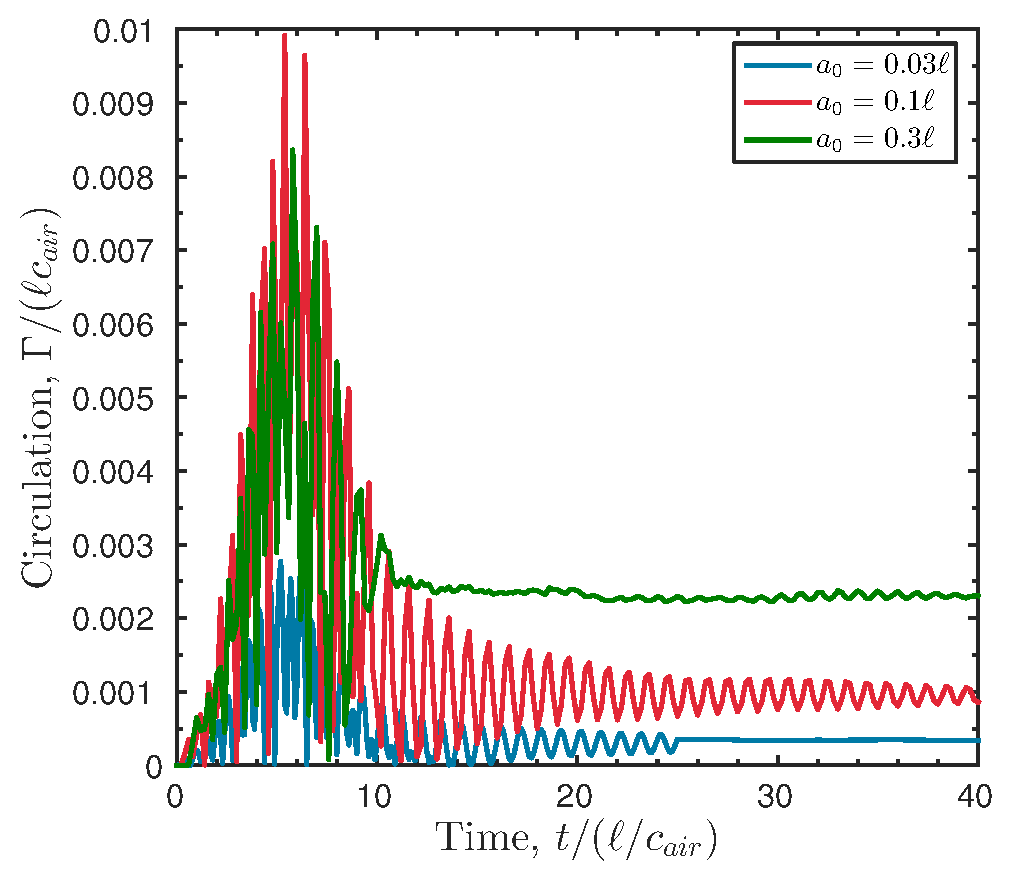
\includegraphics[width=\textwidth]{./figs/lung_figs/rmawave_1_A50_a03,10,30_circulation_01-Mar-2017}
      };%
      \begin{scope}[x={(image.south east)},y={(image.north west)}]%
        \node[font=\normalsize,right] at (0.07,0.13) {};%
      \end{scope}%  
    \end{tikzpicture}%
    \caption{\label{fig:us_circulation_a0_dependence} $p_a = 5$ MPa, $a_0 = 0.03\ell, 0.1\ell, 0.3\ell$}
  \end{subfigure}
  ~
  \begin{subfigure}[b]{0.49\textwidth}
    \begin{tikzpicture}%
      \node[anchor=south west,inner sep=0] (image) at (0,0) {
        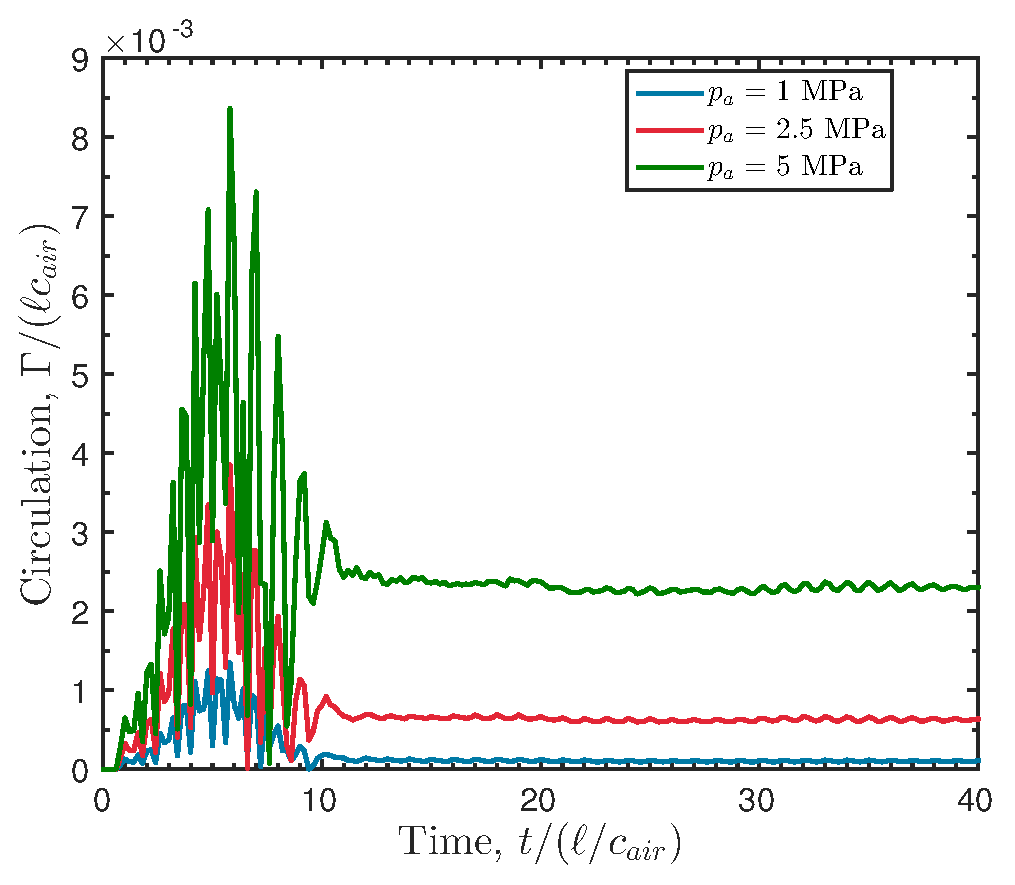
\includegraphics[width=\textwidth]{./figs/lung_figs/rmawave_1_A10,25,50_a30_circulation_01-Mar-2017}
      };%
      \begin{scope}[x={(image.south east)},y={(image.north west)}]%
        \node[font=\normalsize,right] at (0.07,0.13) {};%
      \end{scope}%  
    \end{tikzpicture}%
    \caption{\label{fig:us_circulation_pa_dependence} $p_a = 1, 2.5, 5$ MPa, $a_0 = 0.3\ell$}
  \end{subfigure}
  \caption{Ultrasound-deposited circulation}
  \label{fig:us_circulation_history}
\end{figure}
%
\subsection{Interface strain, $\varepsilon$}
In consideration of strain-induced damage of the alveolar wall, the
linear strain histories $\varepsilon(t)$, as defined in Equation
\eqref{eq:linear_strain}, are plotted for each wave and perturbation
amplitude combination. I will first examine the dependence of strain
on $p_a$ and $a_0$ and then discuss the results in the context of
\ac{DUS}.

To illustrate the dependence of the interface strain on the pulse
amplitude $p_a$, Figure \ref{fig:pa_dependence_strain} plots
$\varepsilon(t)$ for $p_a = 1$ (blue), $2$ (red), and $5$ (green)
MPa. Subfigures \subref{fig:strain_multi-pa_a03},
\subref{fig:strain_multi-pa_a10}, and \subref{fig:strain_multi-pa_a30}
correspond to initial perturbation amplitudes
$a_0 = 0.03\ell, 0.1\ell,$ and $0.3\ell$ respectively. Similarly, to
illustrate the dependence of $\varepsilon$ on the initial perturbation
amplitude $a_0$, Figure \ref{fig:a0_dependence_strain} shows a subset
of this data re-plotted for fixed $p_a$. Strain histories
$\varepsilon(t)$ are shown for $a_0 = 0.03\ell$ (blue), $0.1\ell$
(red), and $0.3\ell$ (green). Subfigures
\subref{fig:strain_multi-a0-A25} and \subref{fig:strain_multi-a0-A50}
correspond to constant $p_a = 2.5$ and $5$ MPa respectively. For all
pressure amplitudes $a_0$ and initial perturbation amplitudes $a_0$,
negative strain is observed during and immediately following the wave
interaction, indicating a net compression of the interface. This
compression is observed to correspond to the flattening of the
interface perturbation during and after the interaction with the
acoustic pulse. For the $p_a = 1$ MPa wave and all $a_0$ and the $2.5$
MPa wave with $a_0 = 0.03\ell$ and $0.1\ell$, this compression is
observed to slowly continue at a decreasing rate throughout the
duration of the simulation. For the $p_a = 2.5$ MPa wave with
$a_0 = 0.1\ell$ and the $p_a = 5$ MPa wave and all $a_0$, the
compression is followed by a net expansion or stretching of the
interface at late times. Based on Figures \ref{fig:rho_snapshots_A25}
and \ref{fig:rho_snapshots_A50} we can see this that this corresponds
to the growth of the aforementioned fluid spike. As we observe that
this deformation and strain increase occur long after the passage of
the wave, when the acoustic pressure is $0$, and as such cannot be
explained by linear acoustics.

Unsurprisingly, the strains observed rise with increasing $p_a$ and
$a_0$. The minimal strain case is observed to occur for
$a_0 = 0.03\ell$ and $p_a = 1$ MPa. For this case, the maximum strain
is observed at the final computed time $t = 500$ is
$\varepsilon-0.001$. The maximum strain case occurs for
$a_0 = 0.3\ell$ and $p_a = 5$ MPa. In the interest of increasing the
relevance of the presented work to \ac{DUS}-induced lung hemorrhage we
consider the presented strain results relative to the $8\%$ strain
failure criteria \citep{Vlahakis2000}. For this case, the maximum
strain observed at the final computed time $t = 500$ and is
$\varepsilon+0.38$. For the cases with $a_0 \geq 0.1\ell$ and
$p_a = 5$ MPa the strain exceeds the $\varepsilon=0.08$ threshold at
$t = 171$ and $t = 377$. For a $200 \mu$m alveolus, this would occur
at approximately $100$ and $220 \mu$s.
%
\begin{figure}
  \centering
  \begin{subfigure}[b]{0.49\textwidth}
    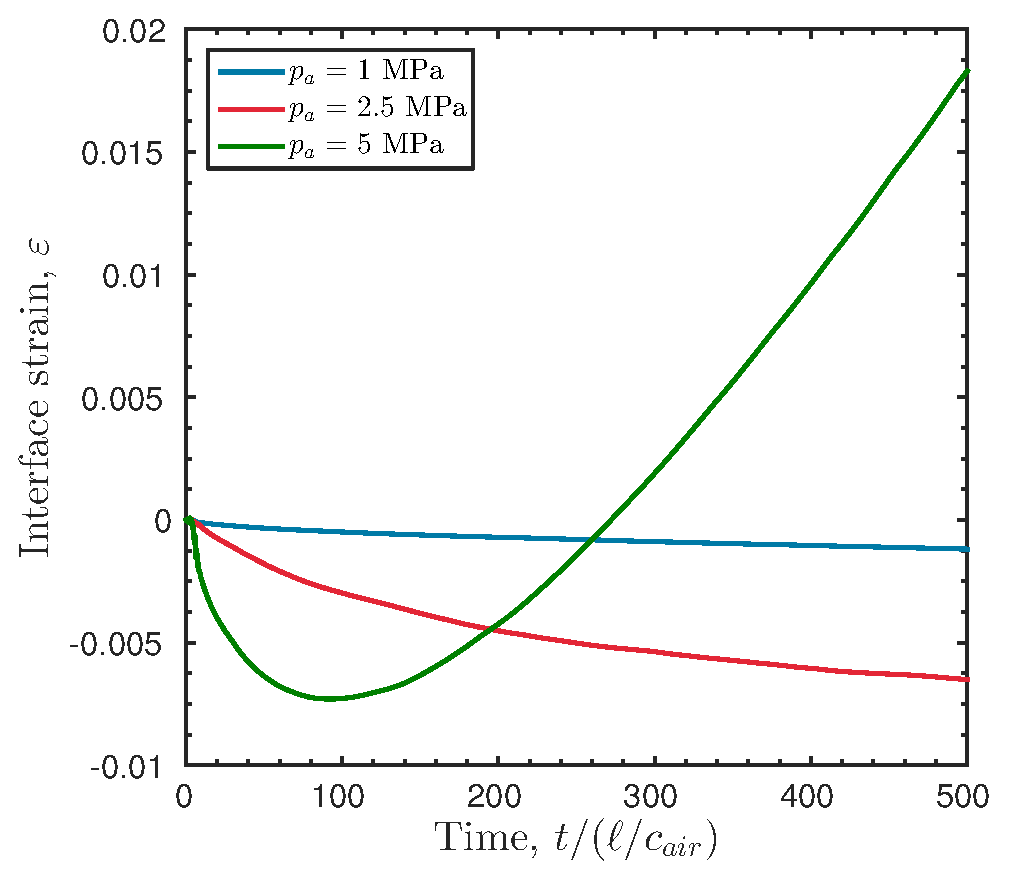
\includegraphics[width=\textwidth]{./figs/lung_figs/rmawave_1_A10,25,50_a03_strain_08-Mar-2017}
    \caption{\label{fig:strain_multi-pa_a03} $a_0 = 0.03\ell$}
  \end{subfigure}
  ~ 
  \begin{subfigure}[b]{0.49\textwidth}
    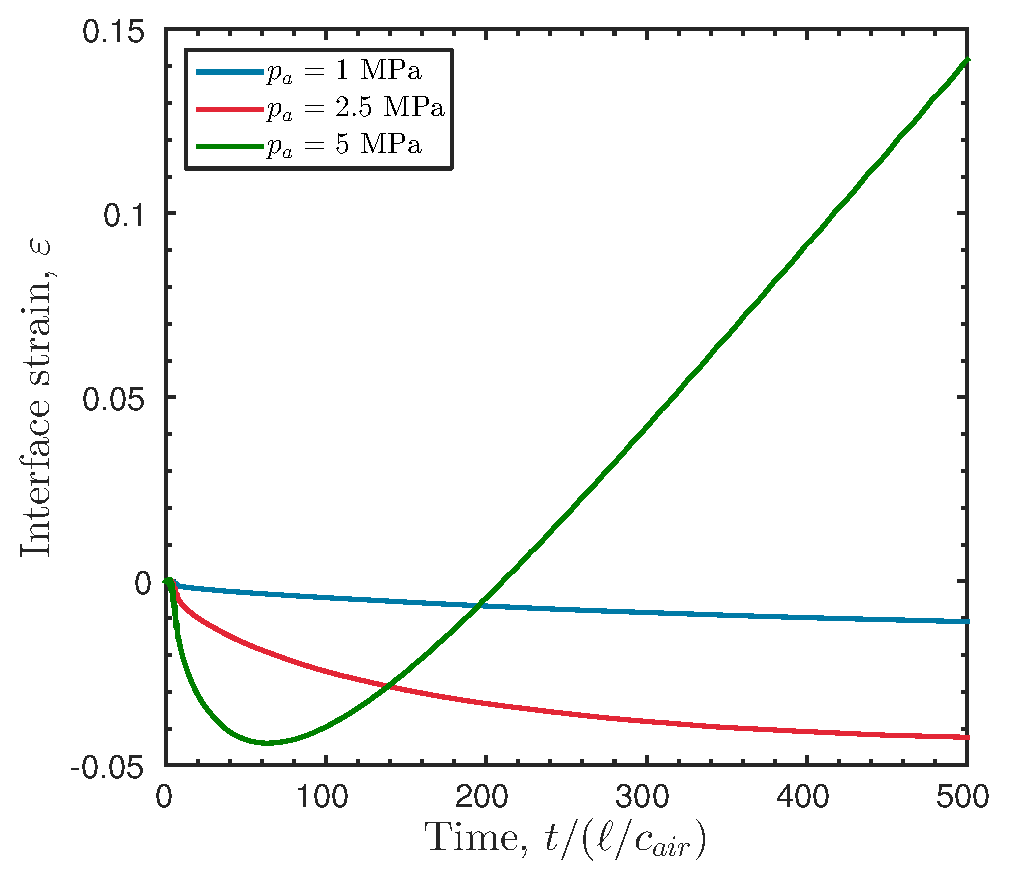
\includegraphics[width=\textwidth]{./figs/lung_figs/rmawave_1_A10,25,50_a10_strain_08-Mar-2017}
    \caption{\label{fig:strain_multi-pa_a10} $a_0 = 0.1\ell$}
  \end{subfigure}
  ~ 
  \begin{subfigure}[b]{0.49\textwidth}
    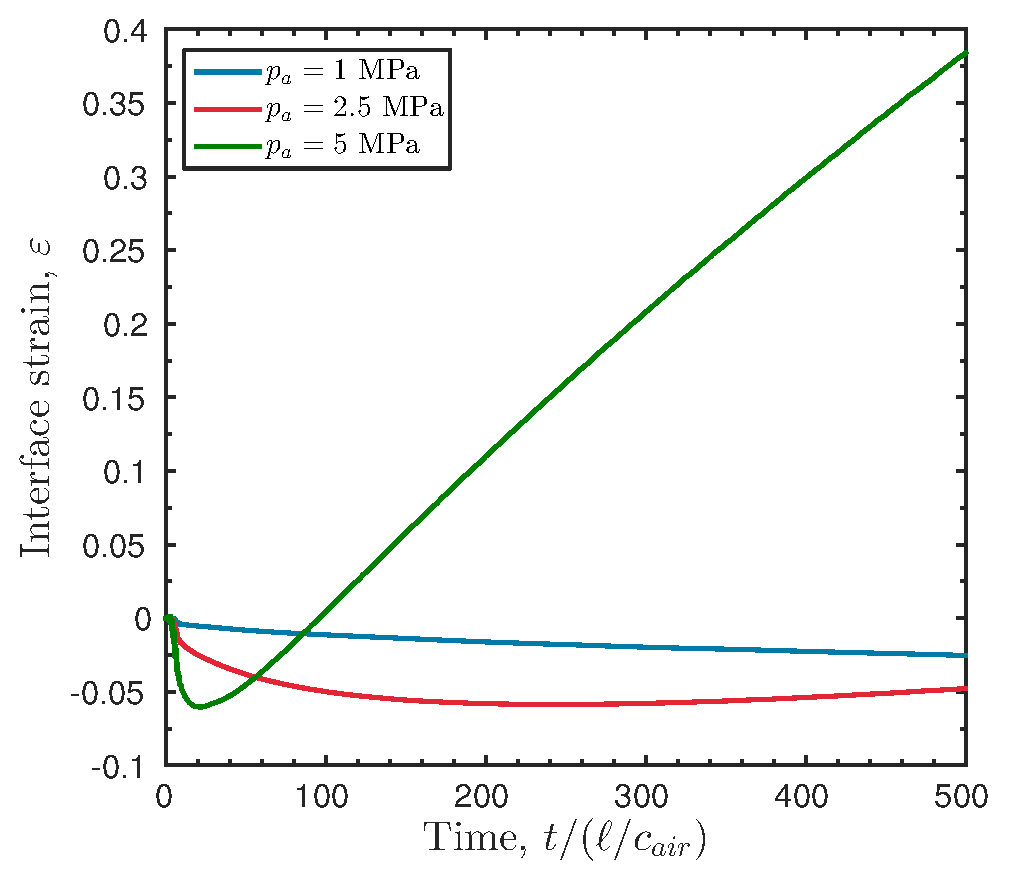
\includegraphics[width=\textwidth]{./figs/lung_figs/rmawave_1_A10,25,50_a30_strain_08-Mar-2017}
    \caption{\label{fig:strain_multi-pa_a30} $a_0 = 0.3\ell$}
  \end{subfigure}
  %
  \caption{To illustrate the dependence of the interface strain on the
    pulse amplitude, the linear strain is plotted as a function of
    time for $t\leq500$ for $p_a=1, 2.5,$ and $5$ MPa pulses. Each plot
    shows $\varepsilon$ for a different initial
    condition. In Figures \subref{fig:strain_multi-pa_a03},
    \subref{fig:strain_multi-pa_a10}, and
    \subref{fig:strain_multi-pa_a30} $a_0=0.03\ell,\, 0.1\ell,$ and
    $0.3\ell$ respectively.}
 \label{fig:pa_dependence_strain}
\end{figure}
%
\begin{figure}
  \centering
  \begin{subfigure}[b]{0.49\textwidth}
    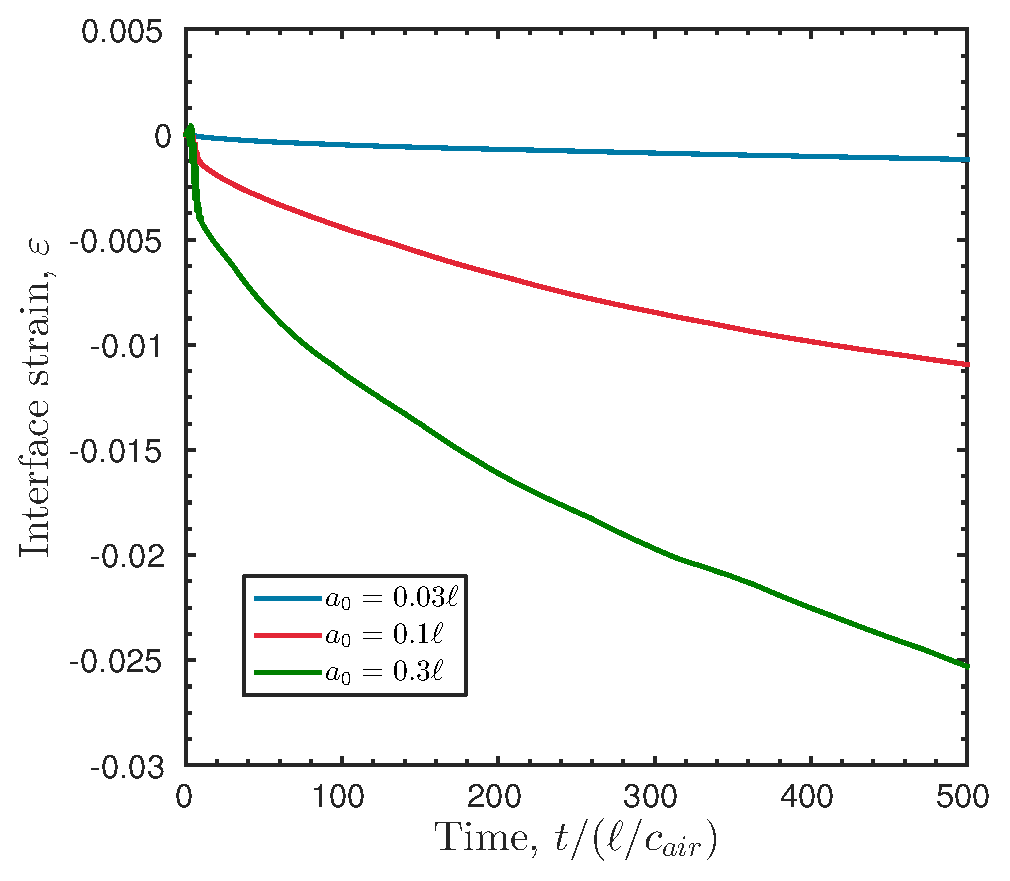
\includegraphics[width=\textwidth]{./figs/lung_figs/rmawave_1_A10_a03,10,30_strain_08-Mar-2017}
    \caption{\label{fig:strain_multi-a0-A10} $p_a = 1.0$ MPa}
  \end{subfigure}
  ~ 
  \begin{subfigure}[b]{0.49\textwidth}
    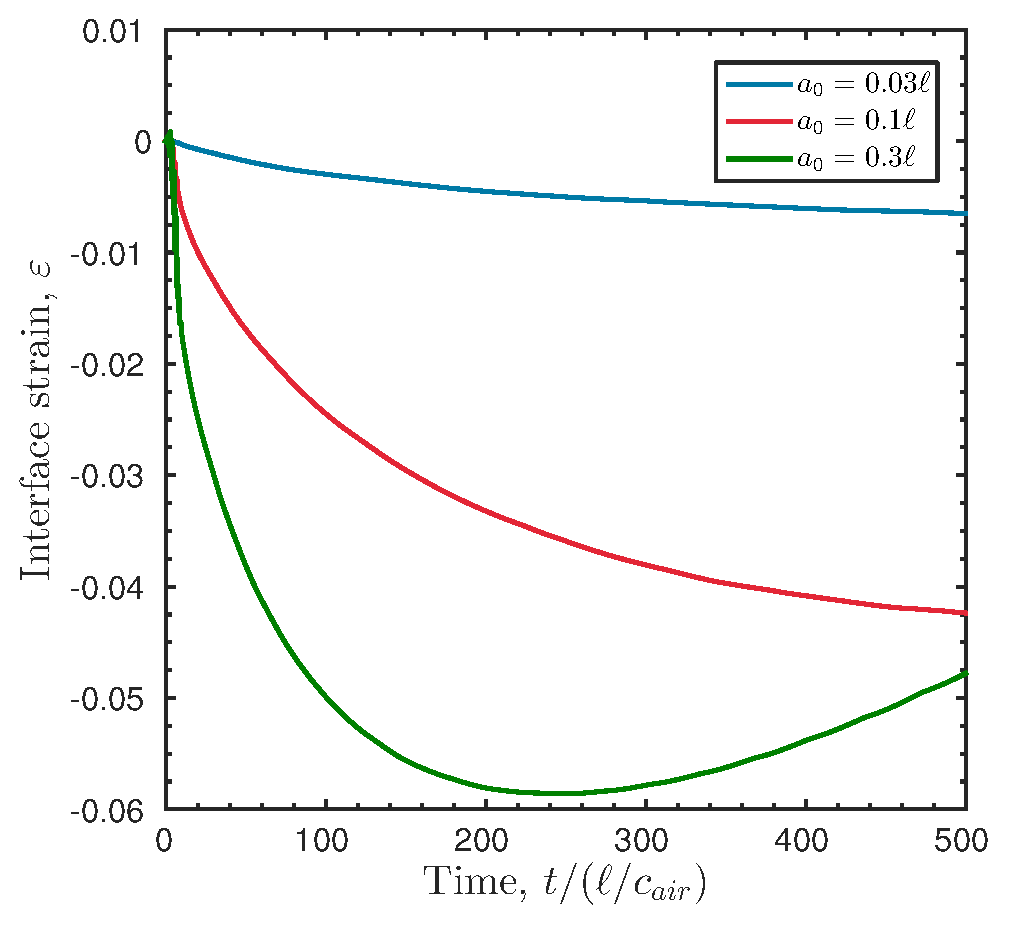
\includegraphics[width=\textwidth]{./figs/lung_figs/rmawave_1_A25_a03,10,30_strain_08-Mar-2017}
    \caption{\label{fig:strain_multi-a0-A25} $p_a = 2.5$ MPa}
  \end{subfigure}
  ~
  \begin{subfigure}[b]{0.49\textwidth}
    \includegraphics[width=\textwidth]{./figs/lung_figs/rmawave_1_A50_a03,10,30_strain_08-Mar-2017}
    \caption{\label{fig:strain_multi-a0-A50} $p_a = 5$ MPa}
  \end{subfigure}
  % 
  \caption{To illustrate the dependence of the interface strain on the
    initial interface amplitude $a_0$, the linear strain of the
    interface is plotted as a function of time for $t\leq500$ for
    $a_0=0.03\ell, 0.1\ell,$ and $0.3\ell$. Each plot shows $\varepsilon$
    for a different pulse amplitude $p_a$. Figure
    \subref{fig:stress_multi-a0-A25}, $p_a = 2.5$ MPa and in Figure
    \subref{fig:stress_multi-a0-A50}, $p_a = 5$ MPa .}
  \label{fig:a0_dependence_strain}
\end{figure}
%
%
\subsection{Viscous stress}
In consideration of the viscous stress we are primarily interested in
the potential for viscous stress-related damage of the alveolar
walls. Thus we consider the point along the interface, at which the
viscous stress is greatest. We observe, somewhat unsurprisingly, that
this stress occurs during the wave-interface interaction, and in
particular occurs near the point when the maximum pressure amplitude
encounters the interface. To illustrate the viscous stress around the
interface color contours of the viscous stress fields are provided for
the $p_a = 5$ MPa case in Figure \ref{fig:tauxy_snapshots} at $t=5$,
approximately when the acoustic pulse and viscous stress are at their
maximum amplitudes. Subfigures \ref{fig:tauxy_snapshot_A50_a03},
\ref{fig:tauxy_snapshot_A50_a10}, and \ref{fig:tauxy_snapshot_A50_a30}
again correspond to respective initial perturbation amplitudes of
$a_0 = 0.03\ell, 0.1\ell,$ and $0.3\ell$. Black lines indicate
isocontours of the volume fraction of water $y_0 = 0.5$. The maximum
viscous stress is observed to occur in the lighter region of the
interface, in which the fluid is mostly made up of air and the
velocity gradients are higher. At this point in time, the fluid around
the interface has had little time to accelerate as a result of the
wave and consequently the interface remains largely undeformed.

For each of the initial perturbation amplitudes $a_0$, Figure
\ref{fig:pa_dependence_stress} shows the maximum viscous stress
amplitude $\abs{\tau_{xy}}_{max}$ in the field as a function of time
for $p_a = 1$ (blue), $2.5$ (red),and $5$ (green) MPa pulses. During
the wave interaction, $\abs{\tau_{xy}}_{max}$ oscillates with the wave
around a mean value which appears to rise and fall with the acoustic
intensity. For a given $a_0$, barring chronologically local
oscillations, $\abs{\tau_{xy}}_{max}$ increases with increasing $p_a$,
i.e, stronger waves. As $a_0$ is varied for fixed $p_a$, two effects
are observed. First, as $a_0$ increases, the maximum viscous stress
appears less oscillatory, or more precisely, the amplitude of
oscillations in $\abs{\tau_{xy}}_{max}$ relative to the chonologically
local mean, decreases. As a result of the varying degree of
oscillation, the second observation is slightly less obvious from the
figures, which is that as $a_0$ increases, the chronologically local
mean value of $\abs{\tau_{xy}}_{max}$ appears to increase with
increasing $a_0$ as well. After the passage of the wave, the maximum
shear stress drops to nearly zero in all cases.

In consideration of \ac{DUS}, we note that for the parameters
considered here the maximum viscous stress amplitudes observed at the
interface occurred during the interaction with the wave and ranged
from $2 < \left|\tau_{xy}\right| \leq 58$ Pa. This is two orders of
magnitude below the $8$ kPa minimal stress failure threshold observed
by \cite{West1991} for disruption of alveolar epithelium. These
stresses occurred during the wave-interface interaction, and quickly
fell off thereafter, in much less time than a typical period between
pulses ($\sim 1$ ms). This suggests that viscous stresses are not
likely to quickly accumulate between pulses. A possible, exception to
this could occur if the velocity field were to change significantly as
a result of accumulated vorticity from subsequent \ac{US} pulses and
assessment of the feasibility of this is beyond the scope of this
work.
%
%
\begin{figure}
  \centering
  \begin{subfigure}[b]{0.32\textwidth}
    \begin{tikzpicture}%
      \node[anchor=south west,inner sep=0] (image) at (0,0) {
        \includegraphics[width=\textwidth]{./figs/lung_figs/rmawave_1_A50_a03_t005_tauxy_snapshots}
      };%
      \begin{scope}[x={(image.south east)},y={(image.north west)}]%
        \node[font=\small,right] at (0.75,0.05) {$\tau_{xy}$ (Pa)};%
      \end{scope}%  
    \end{tikzpicture}%
    \caption{\label{fig:tauxy_snapshot_A50_a03} $a_0 = 0.03\ell$}
  \end{subfigure}
  ~ 
  \begin{subfigure}[b]{0.32\textwidth}
    \begin{tikzpicture}%
      \node[anchor=south west,inner sep=0] (image) at (0,0) {
        \includegraphics[width=\textwidth]{./figs/lung_figs/rmawave_1_A50_a10_t005_tauxy_snapshots}
      };%
      \begin{scope}[x={(image.south east)},y={(image.north west)}]%
        \node[font=\small,right] at (0.75,0.05) {$\tau_{xy}$ (Pa)};%
      \end{scope}%  
    \end{tikzpicture}%
    \caption{\label{fig:tauxy_snapshot_A50_a10} $a_0 = 0.1\ell$}
  \end{subfigure}
  ~ 
  \begin{subfigure}[b]{0.32\textwidth}
    \begin{tikzpicture}%
      \node[anchor=south west,inner sep=0] (image) at (0,0) {
        \includegraphics[width=\textwidth]{./figs/lung_figs/rmawave_1_A50_a30_t500_tauxy_snapshots}
      };%
      \begin{scope}[x={(image.south east)},y={(image.north west)}]%
        \node[font=\small,right] at (0.75,0.05) {$\tau_{xy}$ (Pa)};%
      \end{scope}%  
    \end{tikzpicture}%
    \caption{\label{fig:tauxy_snapshot_A50_a30} $a_0 = 0.3\ell$}
  \end{subfigure}
  % 
  \caption{Contour plots of the Newtonian viscous stress $\tau_{xy}$
    in Pascals are shown for each initial perturbation amplitude for
    the $p_a=5$ MPa pulse at $t=5$, near the point when the maximum
    stress occurs. In Figures \subref{fig:tauxy_snapshot_A50_a03},
    \subref{fig:tauxy_snapshot_A50_a10}, and
    \subref{fig:tauxy_snapshot_A50_a30} $a_0=0.03\ell,\, 0.1\ell,$ and
    $0.3\ell$ respectively.  }
  \label{fig:tauxy_snapshots}
\end{figure}
% 
\begin{figure}
  \centering
  \begin{subfigure}[b]{0.49\textwidth}
    %\includegraphics[width=\textwidth]{./figs/lung_figs/rmawave_1_A10,25,50_a3_tauxy_27-Feb-2017}
    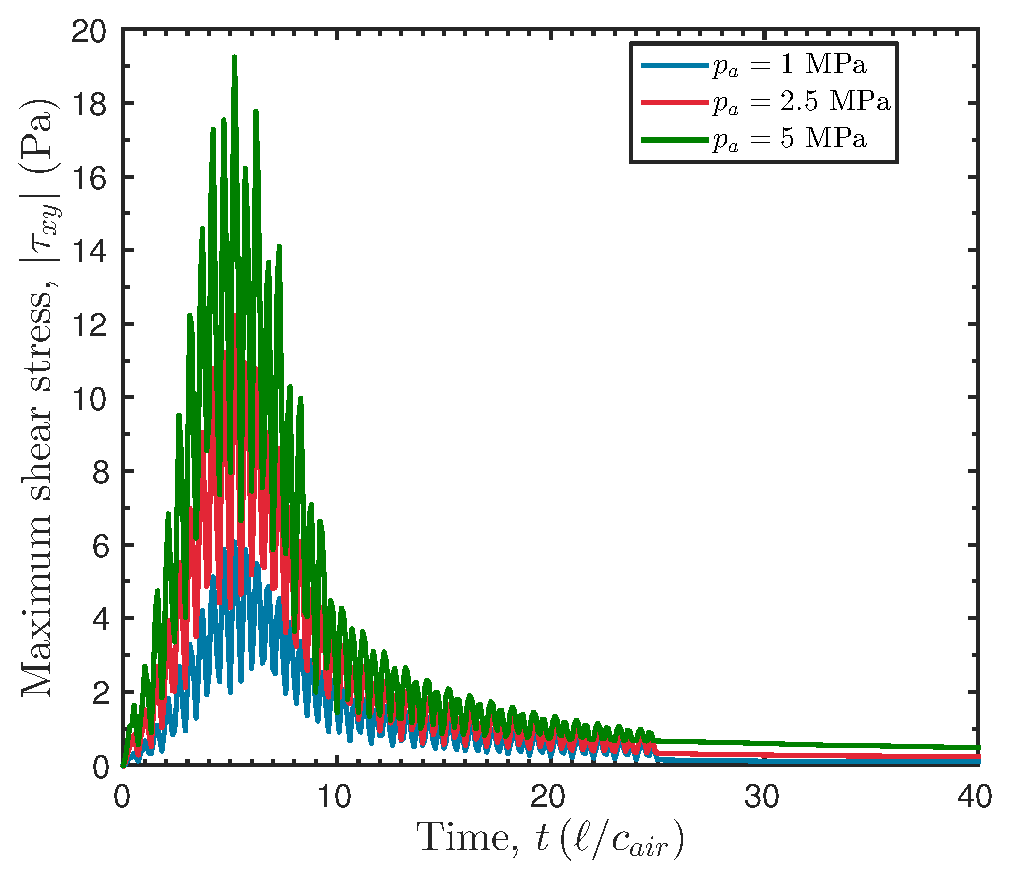
\includegraphics[width=\textwidth]{./figs/lung_figs/rmawave_1_A10,25,50_a03_tauxy_07-Mar-2017}
    \caption{\label{fig:stress_multi-pa_a03} $a_0 = 0.03\ell$}
  \end{subfigure}
  ~ 
  \begin{subfigure}[b]{0.49\textwidth}
    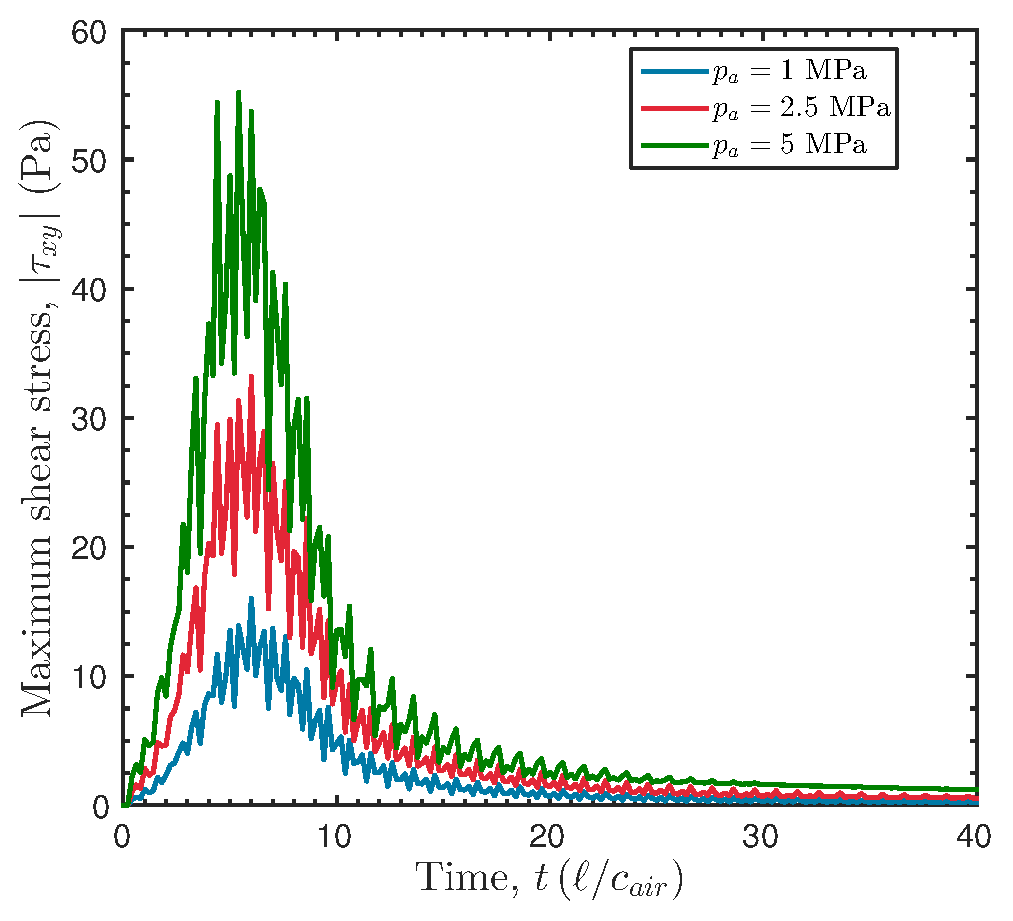
\includegraphics[width=\textwidth]{./figs/lung_figs/rmawave_1_A10,25,50_a10_tauxy_27-Feb-2017}
    \caption{\label{fig:stress_multi-pa_a10} $a_0 = 0.1\ell$}
  \end{subfigure}
  ~ 
  \begin{subfigure}[b]{0.49\textwidth}
    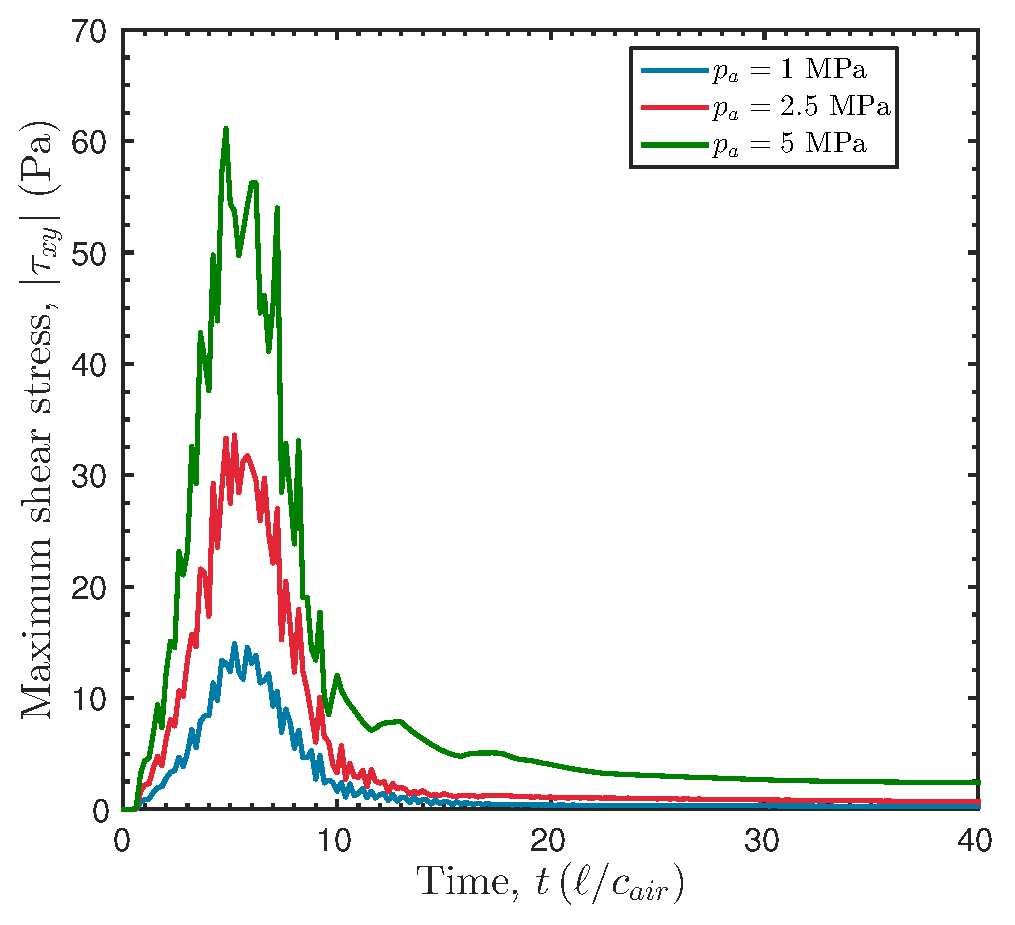
\includegraphics[width=\textwidth]{./figs/lung_figs/rmawave_1_A10,25,50_a30_tauxy_27-Feb-2017}
    \caption{\label{fig:stress_multi-pa_a30} $a_0 = 0.3\ell$}
  \end{subfigure}
  % 
  \caption{To illustrate the dependence of the viscous stress on the
    pulse amplitude, the Maximum shear stress in the field is is
    plotted as a function of time for $t\leq40$ for $p_a=1, 2.5,$ and
    $5$ MPa pulses. Each plot shows $\left|\tau_{xy}\right|_{max}$ for
    a different initial condition. In Figures
    \subref{fig:stress_multi-pa_a03},
    \subref{fig:stress_multi-pa_a10}, and
    \subref{fig:stress_multi-pa_a30} $a_0=0.03\ell,\, 0.1\ell,$ and
    $0.3\ell$ respectively.}
  \label{fig:pa_dependence_stress}
\end{figure}
%
\begin{figure}
  \centering
  \begin{subfigure}[b]{0.49\textwidth}
    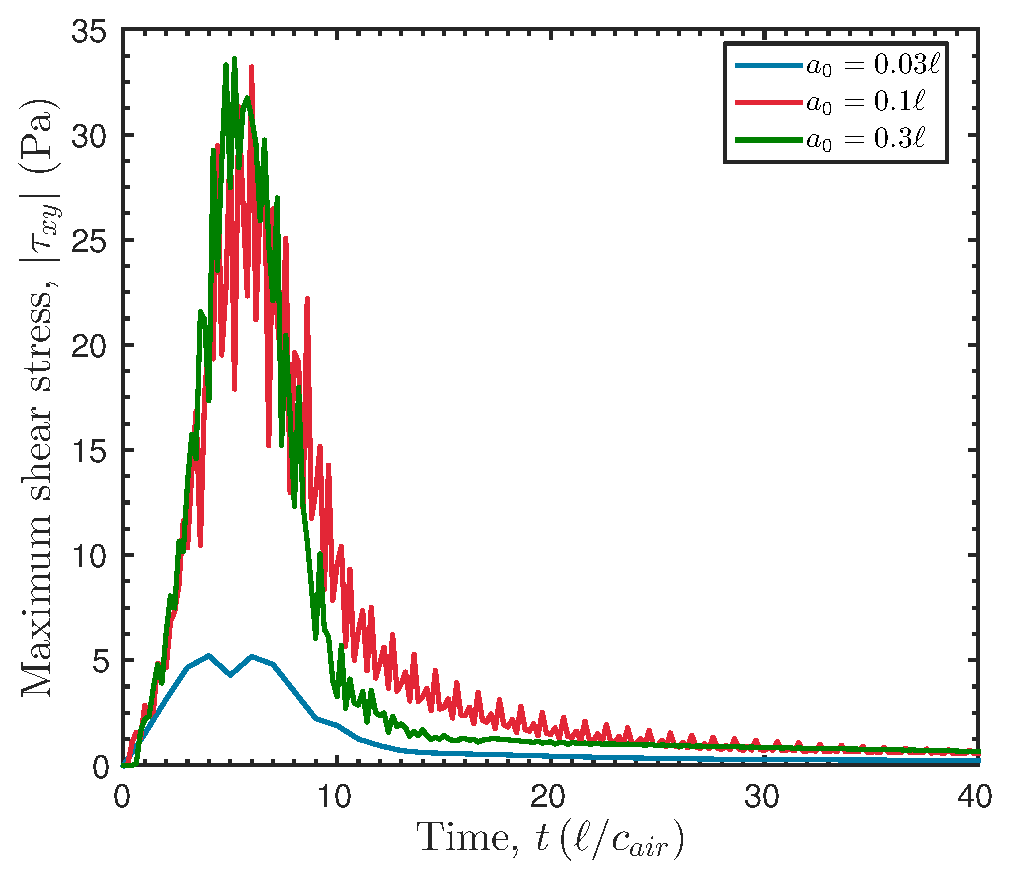
\includegraphics[width=\textwidth]{./figs/lung_figs/rmawave_1_A25_a3,10,30_tauxy_27-Feb-2017}
    \caption{\label{fig:stress_multi-a0-A25} $p_a = 2.5$ MPa}
  \end{subfigure}
  ~ 
  \begin{subfigure}[b]{0.49\textwidth}
    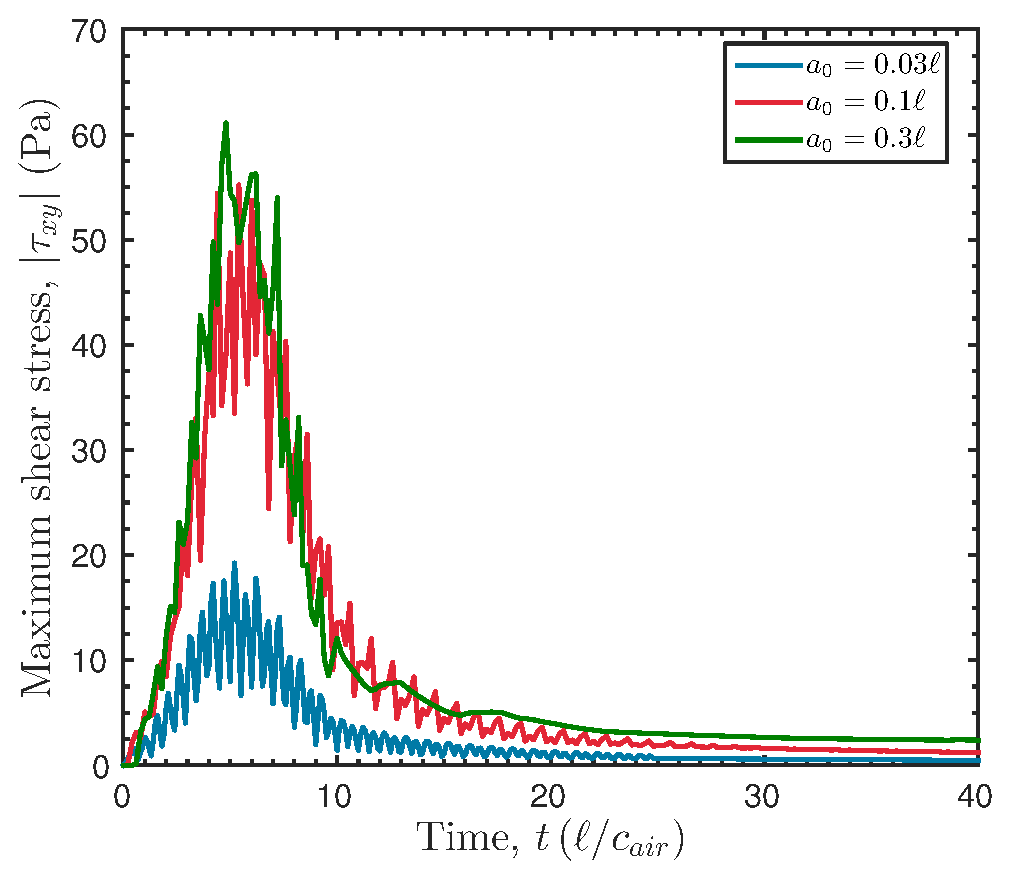
\includegraphics[width=\textwidth]{./figs/lung_figs/rmawave_1_A50_a3,10,30_tauxy_27-Feb-2017}
    \caption{\label{fig:stress_multi-a0-A50} $p_a = 5$ MPa}
  \end{subfigure}
  % 
  \caption{To illustrate the dependence of the viscous stress on the
    initial interface amplitude $a_0$, the Maximum shear stress in the
    field is plotted as a function of time for $t\leq40$ for
    $a_0=0.03\ell, 0.1\ell,$ and $0.3\ell$. Each plot shows
    $\left|\tau_{xy}\right|_{max}$ for a different pulse amplitude $p_a$. In
    Figure \subref{fig:stress_multi-a0-A25}, $p_a = 2.5$ MPa and in
    Figure \subref{fig:stress_multi-a0-A50}, $p_a = 5$ MPa .}
  \label{fig:a0_dependence_stress}
\end{figure}
%
%
%
%

\subsection{Results summary and further Discussion}
\label{sec:usbe_lung_bio}
In summary, \ac{US} pulse waves were simulated propagating from water
into sinusoidal air-water interfaces to model a single \ac{US}-pulse
impinging upon an alveolus from surrounding soft tissue. Nine cases
were considered in which pulses of peak pulse amplitudes of
$p_a = 1, 2.5,$ and $5$ MPa pulses were each propagated at interfaces
of perturbation amplitude $a_0= 0.03\ell, 0.1\ell,$ and $0.3\ell$. For
a typical alveolar size of $200 \mu$m, the maximum simulation time was
approximately $300 \mu$s. Relevant calculations of the density fields,
viscous stress fields, vorticity fields, and interface strain within
the simulated period are reported. For each case, vorticity was
observed to be generated at the interface by the wave-interface
interaction with varying amounts of total circulation remaining after
the passage of the wave. The interfaces continued to deform after the
passage of the wave. The computed peak interface strain amplitudes
ranged from $0.01 \leq \varepsilon \leq 0.38$. Only for the $5$ MPa
did a single pulse induce strains exceeding the 8\% threshold
\citep{Vlahakis2000} during the computed period. The computed peak
stresses were of order $\sim\orderof{Pa}$, far below the $8$ kPa
stress failure criterion \citep{West1991}.

This work is a first step toward investigating the possibility of
baroclinic vorticity in the lungs as potential mechanism of
ultrasound-induced alveolar hemorrhage. However, the approximation of
the alveolar wall as a Newtonian fluid with properties estimated
between air and water does not capture the true complexity of the
system.  As such, there are unsurprisingly several limitations to this
study that do not allow the simulated physics to fully capture the
physics of diagnostic ultrasound-alveolar interactions. These
limitations, include but are not limited to: a simplification of the
geometry that does not capture the inhomogeneity or 3D nature of the
physical problem; physical effects including such as surface tension,
elasticity, viscosity, and heat transfer are neglected; the use of a
single ultrasound pulse is used instead of many consecutive pulses, as
occurs in diagnostic ultrasound.

Based on our physical understanding understanding, it is not
unreasonable to speculate about how each of these limitations is
likely to effect the simulated physics. While the geometry used in
this study is overly simple, it also reflects what could be as a
\textit{best case scenario} in terms of baroclinic vorticity
generation. The orientation of the mean interface and small
perturbation amplitudes relative to what is actually seen in alveoli
create a somewhat minimal misalignment between the interface density
gradient and \ac{US} pressure gradient, resulting in potentially less
baroclinic vorticity generation for a given wave than might be
expected. The physical effects neglected largely work in favor of
increasing the simulated baroclinic vorticity and subsequently driven
interface growth. We expect that viscous effects will dissipate the
kinetic energy of the observed vorticies as heat. However the
timescales over which this dissipation occurs are \hl{FIGURE THIS
  OUT}. The elasticity of the alveolar wall is expected to induce an
elastic stress in the wall, compression, followed by tension based on
the observed strain curves, which will resist the motion of the
wall. While this tensile stress may be an additional mechanism of
damage, the strain in the alveolar wall is likely to be less than
calculated here. \hl{SURFACE TENSION} Additionally, this model does not allow for the
possibility of mechanical failure of the interface and resulting
discontinuities and hemorrhage into the alveolar space. 

Based on our observed results the use of many sequential pulses in
physical diagnostic ultrasound is one that may have significant impact
on the vorticity and interface dynamics. As we have observed in our
work, vorticity left after the passage of the ultrasound led to
significant deformation of the interface, over time periods far less
than the time periods that occur between subsequent \ac{US}
pulses. The potential for accumulation of vorticity, and increased
deformation seems plausible based on our results. The ability to
capture failure behavior is likely to be particularly important in the
case multiple pulses with more realistic geometries, because failure
of the interface and subseqent hemorrhage into the alveolar airspace
may allow for a means by which ultrasound-induced hemorrhage can
propagate into additional alveolar layers.

In addition to the limitations of the present work, there are
definitive limitations of the existing body of knowledge on the
mechanical properties and failure behavior of alveolar tissue under
stresses and strains within the ultrasonic regimes. Poor
characterization of the viscoelastic behavior of alveolar walls makes
determining which physical effects govern the behavior of the system
uncertain. Additionally, the available stress and strain failure
criteria for alveoli are based on much slower processes than occur
during \ac{DUS}, making for an imperfect comparison at best.

%%%%%%%%%%%%%%%%%%%%%%%%%%%%%%% 
\section{conclusions and future work}
While the calculated stresses and strains observed based the
interaction between an air water interface and a single ultrasound
pulse may be representative of a portion the of the physics associated
with \ac{DUS}-alveolar interactions, we cannot confidently say that
baroclinic vorticity is the likely cause of \ac{DUS}-induced
hemorrhage in the lung. We can however draw \hl{three} conclusions from this work. 
\begin{enumerate}
\item Newtonian, viscous stress alone is unlikely to be sufficient to cause \ac{DUS}-induced hemorrhage of the alveolar wall.
\item \ac{DUS} pulses within clinically relevant regimes have the potential to deposit baroclinic vorticity within gas-liquid interfaces in the lungs.
\item \hl{Vorticity may be capable of deforming gas-liquid interfaces in the lungs.}
\end{enumerate}












% \begin{comment}
%   % \section{Results and discussion}
%   % \subsection{Stresses and strains in the lungs}
%   % Lung tissue has been recognized to exhibit viscoelastic behavior
%   % since as early as 1939 \citep{Bayliss1939}. As a result of this,
%   % we consider both viscous and elastic stress as potential damage
%   % mechanisms underlying ultrasound-induced lung hemorrhage.

%   % \subsubsection{Viscous Stresses}
%   % \begin{figure}
%   %   \centering
%   %   \includegraphics{./figs/placeholder}
%   %   \caption{Plot of maximum viscous stress vs time for US pulse
%   %   waveforms.}
%   % \end{figure}

%   % \subsubsection{Elastic Stresses}
%   % \begin{figure}
%   %   \centering
%   %   \includegraphics{./figs/placeholder}
%   %   %   \caption{Plot of engineering strain vs time. Strain on left
%   %   %   side, stress on right side, dashed line at 500 kPa, which is
%   %   %   failure based on \cite{West1999}.}
%   % \end{figure}
% \end{comment}


% \begin{comment} %This is pretty much all in the previous chapter
%   The physical mechanisms underlying \ac{DUS}-induced \ac{PH} are not
%   well understood and traditionally expected \ac{US} bioeffects
%   mechanisms do not appear to be the primary cause of damage. \ac{US}
%   bioeffects mechanisms are typically classified as thermal or
%   non-thermal with the bulk of non-thermal bioeffects being a result
%   of acoustic \ac{IC}. \cite{Zachary2006} finds that \ac{DUS}-induced
%   lung lesions do not appear similar to those induced by heat and
%   concludes that thermal mechanisms are not likely to be the
%   cause. \cite{OBrien2000} observes that the severity of
%   \ac{DUS}-induced \ac{LH} in mice increases under raised hydrostatic
%   pressure, and \cite{Raeman1996} finds that the \ac{LH} is unaffected
%   by the introduction of \ac{US} contrast agents. Both of these
%   findings are inconsistent with what would be expected of
%   \ac{IC}-induced hemorrhage. One study reports detecting cavitation
%   during \ac{DUS}-lung interaction in rats
%   \cite{Holland1996}. \cite{Tjan2007} considers another potential
%   damage mechanism, that focused \ac{US} may lead to the ejection of
%   droplets capable of puncturing the air-filled sacs within the
%   lung. To investigate this, they perform numerical simulations of as
%   an inviscid, free surface subjected to a Gaussian velocity potential
%   and show show that the proposed droplet ejection may occur under
%   certain circumstances. Similarly, \cite{Simon2012} observed
%   \ac{HIFU} induced atomization of tissue at air interfaces. Despite
%   these efforts, the precise damage mechanism underlying
%   \ac{DUS}-induced \ac{LH} is still unknown.
% \end{comment}

% % This is probably all in the last chapter or the introduction. Just add a paragraph relating the last chapter to this one here
% \begin{comment}
%   Previously there has been extensive research
%   investigating interactions between fluid-fluid interfaces driven by
%   mechanical waves. Much of this work has been motivated by man-made
%   applications such as inertial confinement fusion and astrophysical
%   phenomena such as supernova collapse. Accordingly much of the previous
%   research has focused on shock-accelerated, perturbed interfaces
%   between fluids of different densities
%   \citep{Brouillette2002}. \cite{Taylor1950} performed linear stability
%   analysis for the case of a perturbed interface between two fluids
%   undergoing constant acceleration, e.g., gravity. Taylor found that
%   under certain configurations the interface perturbation
%   grows. \cite{Richtmyer1960} extended this linear analysis to the case
%   of an impulsively accelerated interface to create a model for the
%   initial growth of a shock-driven interface perturbation. Later,
%   \cite{Meshkov1969} experimentally confirmed Ricthmyer's qualitative
%   predictions. Hence the growth of a shock-driven fluid-fluid interface
%   has been labeled as the \ac{RMI}. To lend physical insight into the
%   underlying mechanism behind this, \cite{Hawley1989} demonstrated that
%   this phenomenon could be described using vortex deposition-evolution
%   paradigm. The basic mechanism driving the growth of the perturbation
%   in the case of the \ac{RMI} is baroclinic vorticity created by the
%   misalignment of the pressure gradient across the shock and the density
%   gradient at the interface. Recently \hl{Patterson \& Johnson
%     (submitted, 2016)} performed numerical experiments and analysis to
%   show that for the case of liquid-gas interfaces, acoustic waves may
%   also be capable of depositing sufficient baroclinic vorticity at the
%   interface to cause significant deformation, as a result of the sharp
%   density gradient across the interface.
% \end{comment}


% \begin{comment}
%   % \subsection{Summary}
%   As \ac{DUS} of the lung has been shown to trigger same-day, acute
%   alveolar hemorrhage \cite{Zachary2001}, it is specifically
%   interactions between the an aveolus and a single \ac{DUS} pulse that
%   we consider in this work. To investigate the mechanism underlying this
%   hemorrhage, we develop a numerical model of this problem to compute
%   the expected dynamics of the alveolar air-tissue interface for varying
%   acoustic amplitudes an alveolar geometries. To relate the computed
%   dynamics to lung hemorrhage, we approximate the relevant stresses and
%   strains and compare these results to existing values of the material
%   properties alveolar tissue to assess possible causes of hemorrhage.

%   \hl{OUT OF PLACE:\\
%     This work aims to use numerical simulations to investigate the
%     dynamics associated with the interaction between an ultrasound pulse and
%     an aleolar air-tissue interface. We hypothesize that acoustically
%     generated baroclinic vorticity within the lungs is capable of driving
%     deformation of alveolar air-tissue interfaces to the point of
%     hemorrhage. We model the problem as a sinusoidally perturbed air-water
%     interface driven by a single acoustic pulse and study the subsequent
%     dynamics. Calculated stresses and strains are compared to previously
%     measured failure criteria from the literature.}

% \end{comment}

% % This is the old methods section, that now largely exists in the previous chapter.
% \begin{comment}
%   \section{Methods}
%   In this section we develop a model of \ac{DUS}-alveolus interaction
%   as a compressible fluid system. We then describe in detail the setup
%   of the numerical experiments performed and calculations performed to
%   investigate the problem. 

%   \subsection{A model of \ac{DUS}-alveolus interaction}
%   \hl{COPIED THIS PARAGRAPH TO OTHER PAPER}.  Consider a \ac{DUS} pulse
%   as it travels into the lungs. After passing through layers of soft
%   tissue and fluid, the wave encounters a network of openly connected,
%   air-filled saccules with distinctly irregular surfaces. These are the
%   alveoli. It is the interaction between an incident \ac{US} pulse and
%   the first alveolar tissue-air interface it encounters that we treat
%   here, as shown in figure \ref{fig:alveolar_schematic}.

%   To model the problem, we consider a rectangular domain with a 2D
%   $(x,y)$ cross section containing soft tissue (modeled as water)
%   sitting atop a single alveolus (modeled as air) as illustrated in
%   figure \ref{fig:ic_schematic}. An acoustic pulse is prescribed within
%   the water, above the interface, and allowed to propagate downward
%   ($-y$-direction) toward the air. The alveolus spans the width of the
%   domain, $\ell$. A typical mean aveolar diameters in an adult human is
%   $200 \mu$m \citep{Ochs2004}.

%   To capture the irregular shape of the alveolus, the water-air
%   interface contains a single mode sinusoidal perturbation of amplitude
%   $a_0$ such that the vertical center of the interface is described by,
%   \begin{align} %Not y_interface in the code
%     Y(x,t=0)_{interface} = a_0\sin\left(\frac{2\pi x}{\ell}-\frac{\pi}{2}\right). 
%   \end{align}
%   An interface thickness $\delta=0.08$ is chosen such that at $t=0$, the
%   fluid in the domain above $y\geq Y_{interface}+\delta/2$ is pure
%   water, and below $y\leq Y_{interface}-\delta/2$ is pure air, which a
%   water-air mixture filling the region around the interface. A more
%   detailed treatment of the interface can be found in referred to
%   \hl{(Patterson and Johnsen, 2016)}. To investigate the dependence of
%   the dynamics on the alveolar geometry we will consider multiple
%   interface perturbation amplitudes: $a_0=0.03\ell, 0.1\ell, 0.2\ell,$
%   and $0.3\ell$.

%   The diagnostic ultrasound pulse is modeled as a sinusoidal carrier
%   wave of amplitude $p_a$ and frequency $f$ modulated by a Gaussian
%   Envelope such that,
%   \begin{align}
%     p(x,t_0) = p_a\sin{\left(2\pi f\frac{\left[y-\left(Y_{wave}+L_{wave}\right)\right]}{c}\right)}\exp{\left(-\frac{\left(\left[y-\left(Y_{wave}+L_{wave}/2\right)\right]c\right)^2}{FWHM/\left(2\sqrt{2\ln{\left(2\right)}} \right)}\right)}.%
%   \end{align}
%   The carrier wavelength $\lambda=c_{water}/f$ and the full width of the
%   Gaussian envelope at half of the maximum amplitude $FWHM$ are designed
%   to scale appropriately with respect to $\ell$. Here,
%   $f\approx 1.25 c_{water} / 2\pi \ell$ and $FWHM=15\ell$. For an
%   alveolar length scale of $\ell=200 \mu$m, this corresponds to $f=1.65$
%   MHz and $FWHM=3$ mm. $L_{wave}=45\ell$ is the length of the
%   computational domain, over which the wave is defined to exist and
%   $Y_{wave}$ is $y$-location of the bottom of the wave at $t=0$, which
%   is set to $10a_0$ above the peak of the interface. To consider the
%   dependence of the interface dynamics on pulse amplitude we vary
%   $p_a = 1, 5, 10,$ and $15$ MPa.

%   \subsection{Governing Equations}
%   To simulate the model problem described above we solve equations for
%   conservation of mass, momentum, energy. While it has been long since
%   recognized that tissue exhibits viscoelastic behavior
%   \citep{Bayliss1939}. To simplify things we consider the expected
%   length scale over which viscosity will influence the dynamics,
%   $l_{viscous}$. From dimensional analysis, this scales as
%   $l_{viscous}\sim\sqrt{\nu/(\ell/c)}$. In air at 300 K,
%   $l_{viscous}\sim\orderof{1 \mu\text{m}}$ and in water
%   $l_{viscous}\sim\orderof{0.1 \mu\text{m}}$. In either case we consider
%   that $l_{viscous}<<\ell$. \hl{Furthermore, we consider the relative
%     importance of elasticity and surface tension }

%   \begin{comment}
%     \begin{itemize}
%     \item $c_{air} = 347.2$ m/s
%     \item $c_{water} = 1500$ m/s
%     \item $\nu_{air} = 1.568\times 10^{-5}$ m$^2$/s
%     \item $\nu_{water} = 0.8539\times 10^{-6}$ m$^2$/s
%     \item $G_{alveolar-wall} = 5$ kPa \cite{Cavalcante2005}
%     \item $\sigma_{water}=0.072$ at N/m 298K
%     \item $\rho_{air}=1.1765$ kg/m$^3$
%     \item $\rho_{water}=996$ kg/m$^3$
%     \item if $p_a=1 MPa$:
%       \begin{itemize}
%       \item $u_{acoustic-water}\approx0.6$ m/s
%       \item $u_{acoustic-air}\approx1.2$ m/s
%       \end{itemize}
%     \item $Re=\frac{\rho u}{\nu}$ =
%     \item $We=\frac{\rho u^2 \ell}{\sigma}$ = $(\infty)_{air}$ =
%       $()_{water}$
%     \item $Ca=\frac{\rho u^2}{K}$
%     \end{itemize}
%   \end{comment}

%   \begin{subequations} \label{eq:euler}%
%     \begin{align}%
%       \frac{\partial \rho}{\partial t} + \frac{\partial \left(\rho u\right)}{\partial x} + \frac{\partial \left(\rho v\right)}{\partial y} = 0,\\
%       \frac{\partial \rho u}{\partial t} + \frac{\partial}{\partial x}\left( \rho u^2+p\right)  + \frac{\partial}{\partial y}\left( \rho uv\right) = 0,\\
%       \frac{\partial \rho v}{\partial t} + \frac{\partial}{\partial x}\left( \rho uv\right)  + \frac{\partial}{\partial y}\left( \rho v^2+p\right) = 0,\\
%       \frac{\partial E}{\partial t} + \frac{\partial}{\partial x}\left[u\left(E+p\right)\right] + \frac{\partial}{\partial y}\left[v\left(E+p\right)\right] = 0,
%     \end{align}%
%   \end{subequations}%


%   \subsection{Computational implementation}
%   The Euler equations \eqref{eq:euler} are solved on a rectangular
%   computational grid using Discontinuous Galerkin Methods in space and a
%   fourth order Runge-Kutta time marching scheme as described in
%   (Patterson and Johnsen, 2016 [submitted]). As previously mentioned the
%   width of the computational domain is 1 mean alveolar diameter,
%   $\ell$. The length of the domain is chosen based on two criteria: one
%   - the domain must fully capture the initial acoustic wave and the
%   moving interface throughout the simulation, and two - the domain must
%   be long enough to sufficiently largely eliminate artificial
%   reflections from the boundaries. Thus the computational domain
%   considered for this problem is described by $0\leq x\leq1\ell$ and
%   $-20\ell\leq y\leq 60\ell$. To further help eliminate reflections,
%   grid stretching is implemented at the top and bottom $10\ell$.

%   - Wave
%   \begin{itemize}
%   \item ultrasound is focused to a zone that is at least of order
%     $\lambda$, and $\lambda>>\ell.$
%   \item $k_{y-acoustic}/1.25$
%   \end{itemize}


%   -length scales
% \end{comment}


%%% Local Variables:
%%% mode: latex
%%% TeX-master: t
%%% End:
